\documentclass[12pt,a4paper]{article}
\usepackage[utf8]{inputenc}
\usepackage[T1]{fontenc}
\usepackage{booktabs}
\usepackage{graphicx}
\usepackage{amsmath,amssymb}
\usepackage{geometry}
\usepackage{array}
\usepackage{caption}
\usepackage{subcaption}
\usepackage{hyperref}
\usepackage{siunitx}
\usepackage{xcolor}
\usepackage{tikz}
\usetikzlibrary{shapes.geometric, arrows, positioning, fit, calc}

\geometry{margin=25mm}

\sisetup{inter-unit-product=\cdot}

\hypersetup{
    colorlinks=true,
    linkcolor=blue,
    filecolor=magenta,
    urlcolor=cyan,
}

\pagenumbering{arabic}

\begin{document}

\begin{titlepage}
    \centering
    \vspace*{2cm}
    
    {\LARGE\bfseries Apprentissage par Renforcement Profond pour le Contrôle Automatisé de l'Anesthésie\par}
    \vspace{1.5cm}
    
    {\Large Mohamed Haytam Soukraty\par}
    \vspace{0.5cm}
    
    {\large Avril 2026\par}
    \vspace{2cm}
    
    \begin{abstract}
        \noindent
        Ce travail présente quatre approches d'apprentissage par renforcement pour l'administration automatisée de propofol pendant la chirurgie, utilisant la surveillance BIS et les simulations PK/PD. Les algorithmes vont des méthodes tabulaires (Q-Learning, Programmation Dynamique) au RL profond (DQN), tous opérant sur une représentation floue de la dynamique d'erreur du BIS. Nos résultats indiquent que tous les modèles nécessitent un entraînement supplémentaire pour atteindre une performance cliniquement acceptable, avec Q-Learning montrant le sous-entraînement le plus sévère et les méthodes basées sur la programmation dynamique démontrant une instabilité de contrôle modérée.
    \end{abstract}
    
    \vspace{1.5cm}
    \textbf{Mots-clés:} Apprentissage par Renforcement, Contrôle de l'Anesthésie, Surveillance BIS, Propofol, Modélisation PK/PD
    
\end{titlepage}

\newpage

\section{Introduction}

Le maintien d'une profondeur d'anesthésie adéquate pendant les procédures chirurgicales représente un défi critique en médecine moderne. L'Index Bispectral (BIS) fournit une mesure validée de l'état hypnotique, permettant le contrôle en boucle fermée de l'administration d'anesthésique. Ce travail utilise l'apprentissage par renforcement pour optimiser les taux d'infusion de propofol, avec l'objectif de maintenir le BIS à une valeur cible de 50 tout au long de la chirurgie.

Le modèle de Schnider fournit des simulations pharmacocinétiques et pharmacodynamiques qui capturent les caractéristiques de réponse médicamenteuse spécifiques au patient. Quatre algorithmes d'apprentissage par renforcement distincts sont implémentés et évalués: Q-Learning tabulaire, Itération de Politique par Programmation Dynamique, Itération de Valeur par Programmation Dynamique, et Deep Q-Network (DQN).

\section{Représentation de l'État et Actions}

Tous les algorithmes partagent une représentation d'état floue commune dérivée des mesures BIS. Le vecteur d'état comprend deux composantes:

\begin{equation}
    s = (\text{BIS\_ERROR}, \text{DELTA\_BIS})
\end{equation}

où BIS\_ERROR représente la différence entre le BIS actuel et le BIS cible ($\text{BIS} - \text{BIS}_{\text{target}} \in [-50, +50]$), et DELTA\_BIS capture la dérivée temporelle ($\text{BIS}[t] - \text{BIS}[t-1] \in [-30, +30]$).

Chaque valeur continue undergoes fuzzification utilisant trois fonctions d'appartenance (négatif, zéro, positif), produisant six caractéristiques floues. Discrétisées sur 10 intervalles par caractéristique, ceci crée un espace d'états discret de $10^6$ états.

L'espace d'actions se compose de sept taux d'infusion de propofol discrets:

\begin{equation}
    \mathcal{A} = \{0.0, 0.5, 1.0, 2.0, 3.0, 4.0, 6.0\} \ \text{ml/min}
\end{equation}

\section{Modèles d'Apprentissage par Renforcement}

\subsection{Q-Learning (Tabulaire)}

Q-Learning est un algorithme hors-politique sans modèle qui apprend les valeurs d'action optimales par des mises à jour de différence temporelle. L'agent maintient une table Q de taille $10^6 \times 7$ et sélectionne les actions utilisant une politique $\epsilon$-glouton.

\begin{figure}[htbp]
    \centering
    \begin{tikzpicture}[
        node distance=1.5cm,
        box/.style={rectangle, draw, minimum width=2.5cm, minimum height=1cm, align=center},
        arrow/.style={->, thick},
        >=stealth
    ]
    
    \node (bis) [box] {$\text{BIS}[t]$};
    \node (compute) [box, right=of bis] {Calculer\\BIS\_ERROR,\\DELTA\_BIS};
    \node (fuzzy) [box, right=of compute] {État\\Flou $s$};
    \node (qtable) [box, below=of fuzzy] {Table Q\\$(10^6 \times 7)$};
    \node (selection) [box, below=of qtable] {Sélection $\epsilon$-glouton\\d'Action};
    \node (reward) [box, right=of selection] {$r = -|\text{BIS\_ERROR}|$\\$- 0.5 \times |\text{DELTA\_BIS}|$};
    \node (action) [box, below=of selection] {Action $a$};
    
    \draw[arrow] (bis) -- (compute);
    \draw[arrow] (compute) -- (fuzzy);
    \draw[arrow] (fuzzy) -- (qtable);
    \draw[arrow] (qtable) -- (selection);
    \draw[arrow] (selection) -- (action);
    \draw[arrow] (selection) -- (reward);
    
    \end{tikzpicture}
    \caption{Architecture Q-Learning pour le contrôle de l'anesthésie}
    \label{fig:qlearning}
\end{figure}

La fonction de récompense pénalise à la fois l'erreur BIS absolue et l'oscillation:

\begin{equation}
    r = -|\text{BIS\_ERROR}| - 0.5 \times |\text{DELTA\_BIS}|
\end{equation}

\textbf{Hyperparamètres:} $\text{ÉPISODES} = 1{,}000{,}000$, $\text{PAS} = 120$, $\alpha = 0.2$, $\gamma = 0.69$, $\epsilon = 0.1$

\textbf{Statut d'entraînement:} Nécessite un entraînement supplémentaire. La performance actuelle indique une administration de propofol insuffisante, avec MDPE restant à environ 94.79\%.

\begin{figure}[htbp]
    \centering
    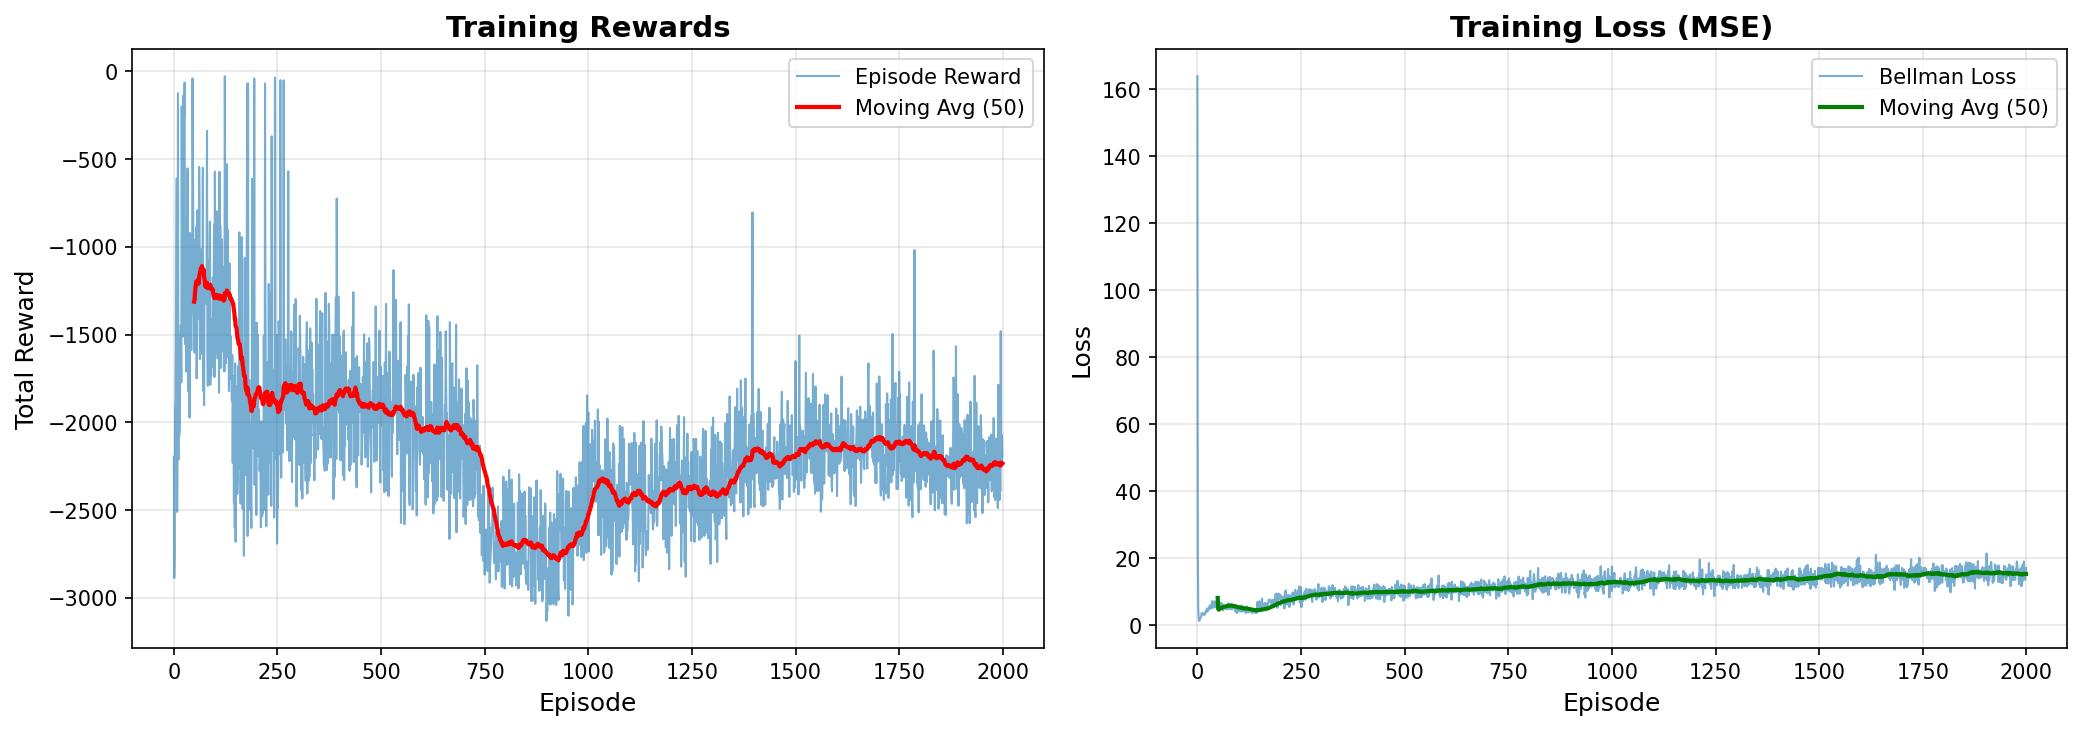
\includegraphics[width=0.85\textwidth]{images/training_curves.png}
    \caption{Convergence de l'entraînement pour l'agent Q-Learning}
    \label{fig:q_training}
\end{figure}

\begin{figure}[htbp]
    \centering
    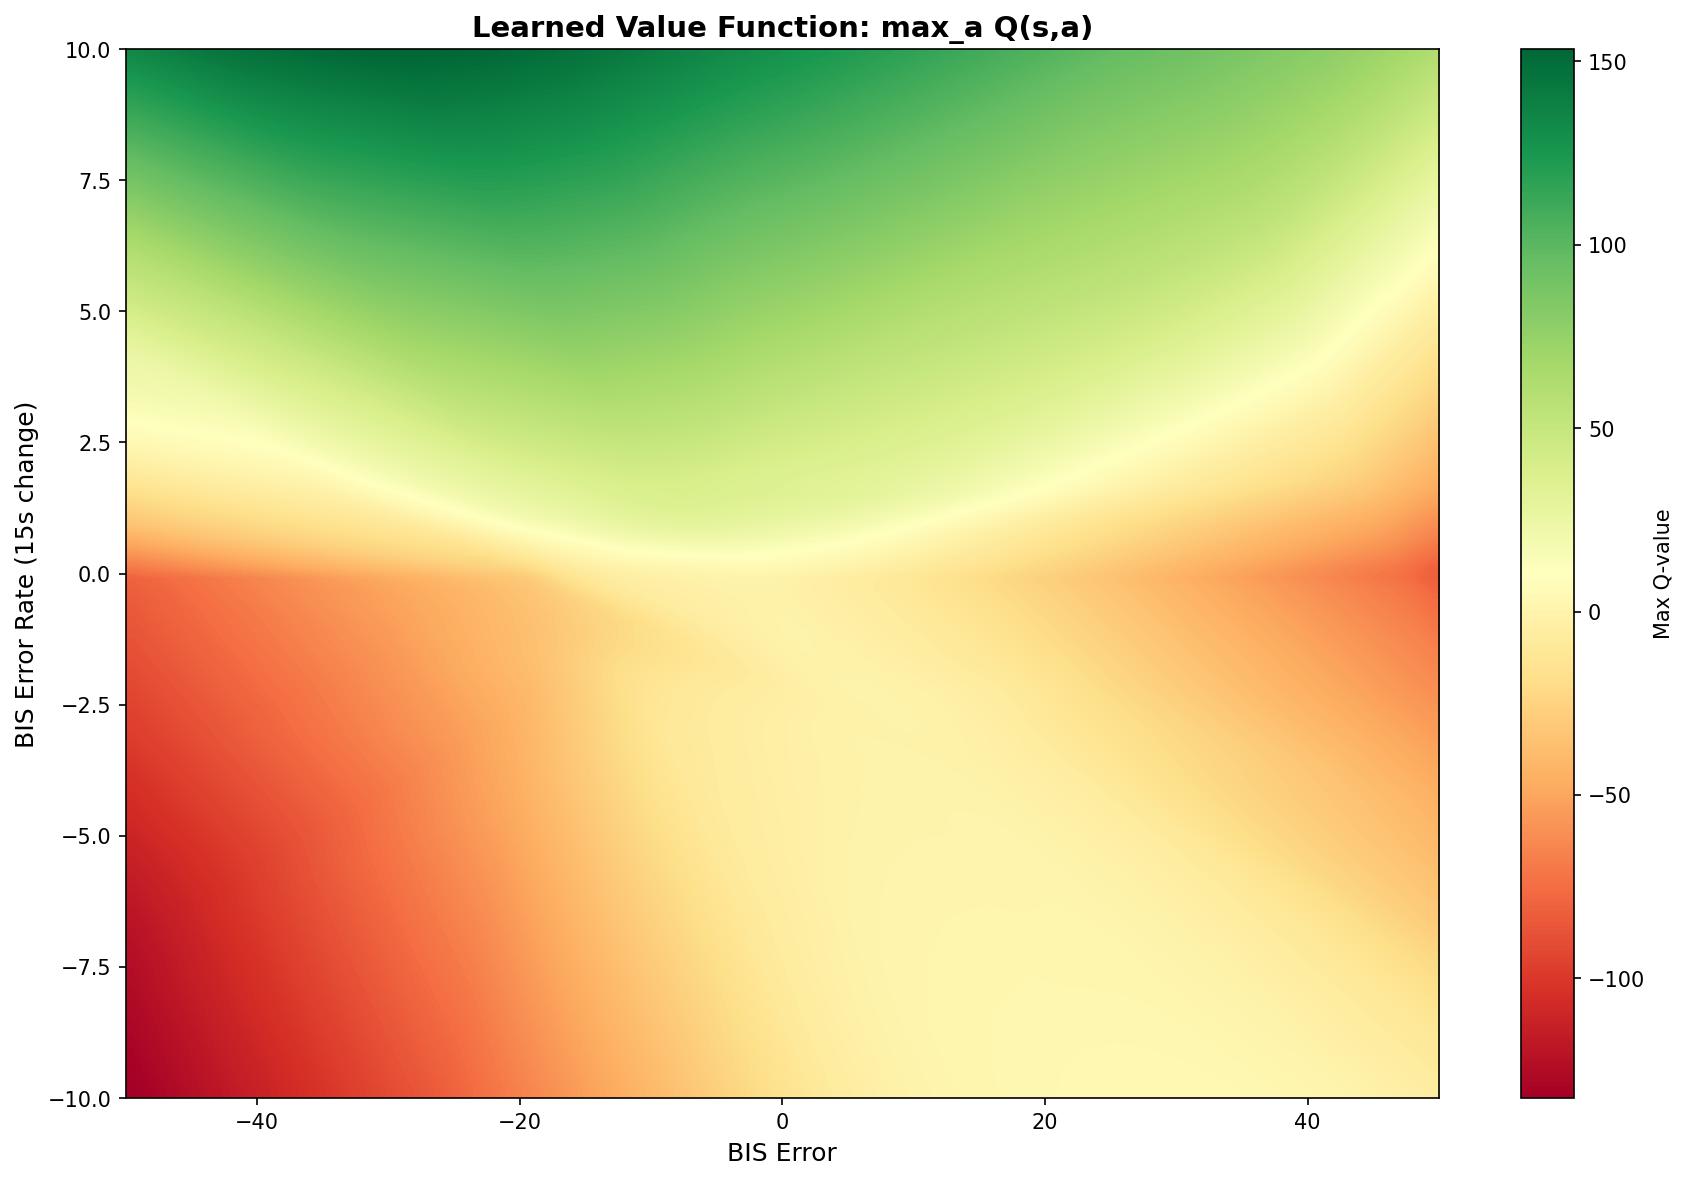
\includegraphics[width=0.85\textwidth]{images/q_values_heatmap.png}
    \caption{Carte thermique des valeurs Q dans l'espace d'états}
    \label{fig:q_heatmap}
\end{figure}

\begin{figure}[htbp]
    \centering
    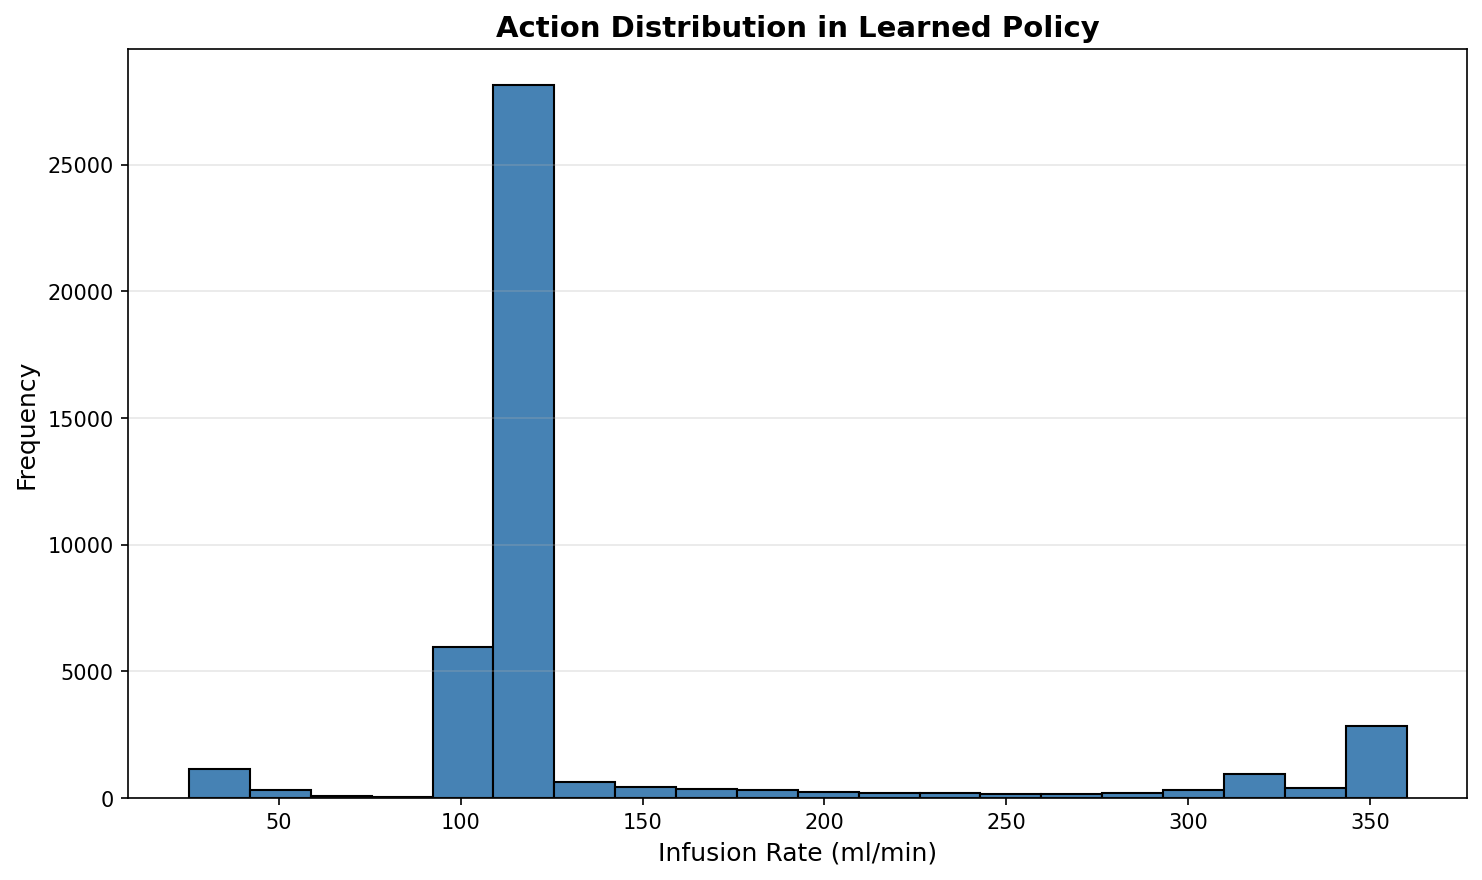
\includegraphics[width=0.85\textwidth]{images/action_distribution.png}
    \caption{Distribution de probabilité des actions}
    \label{fig:action_dist}
\end{figure}

\begin{figure}[htbp]
    \centering
    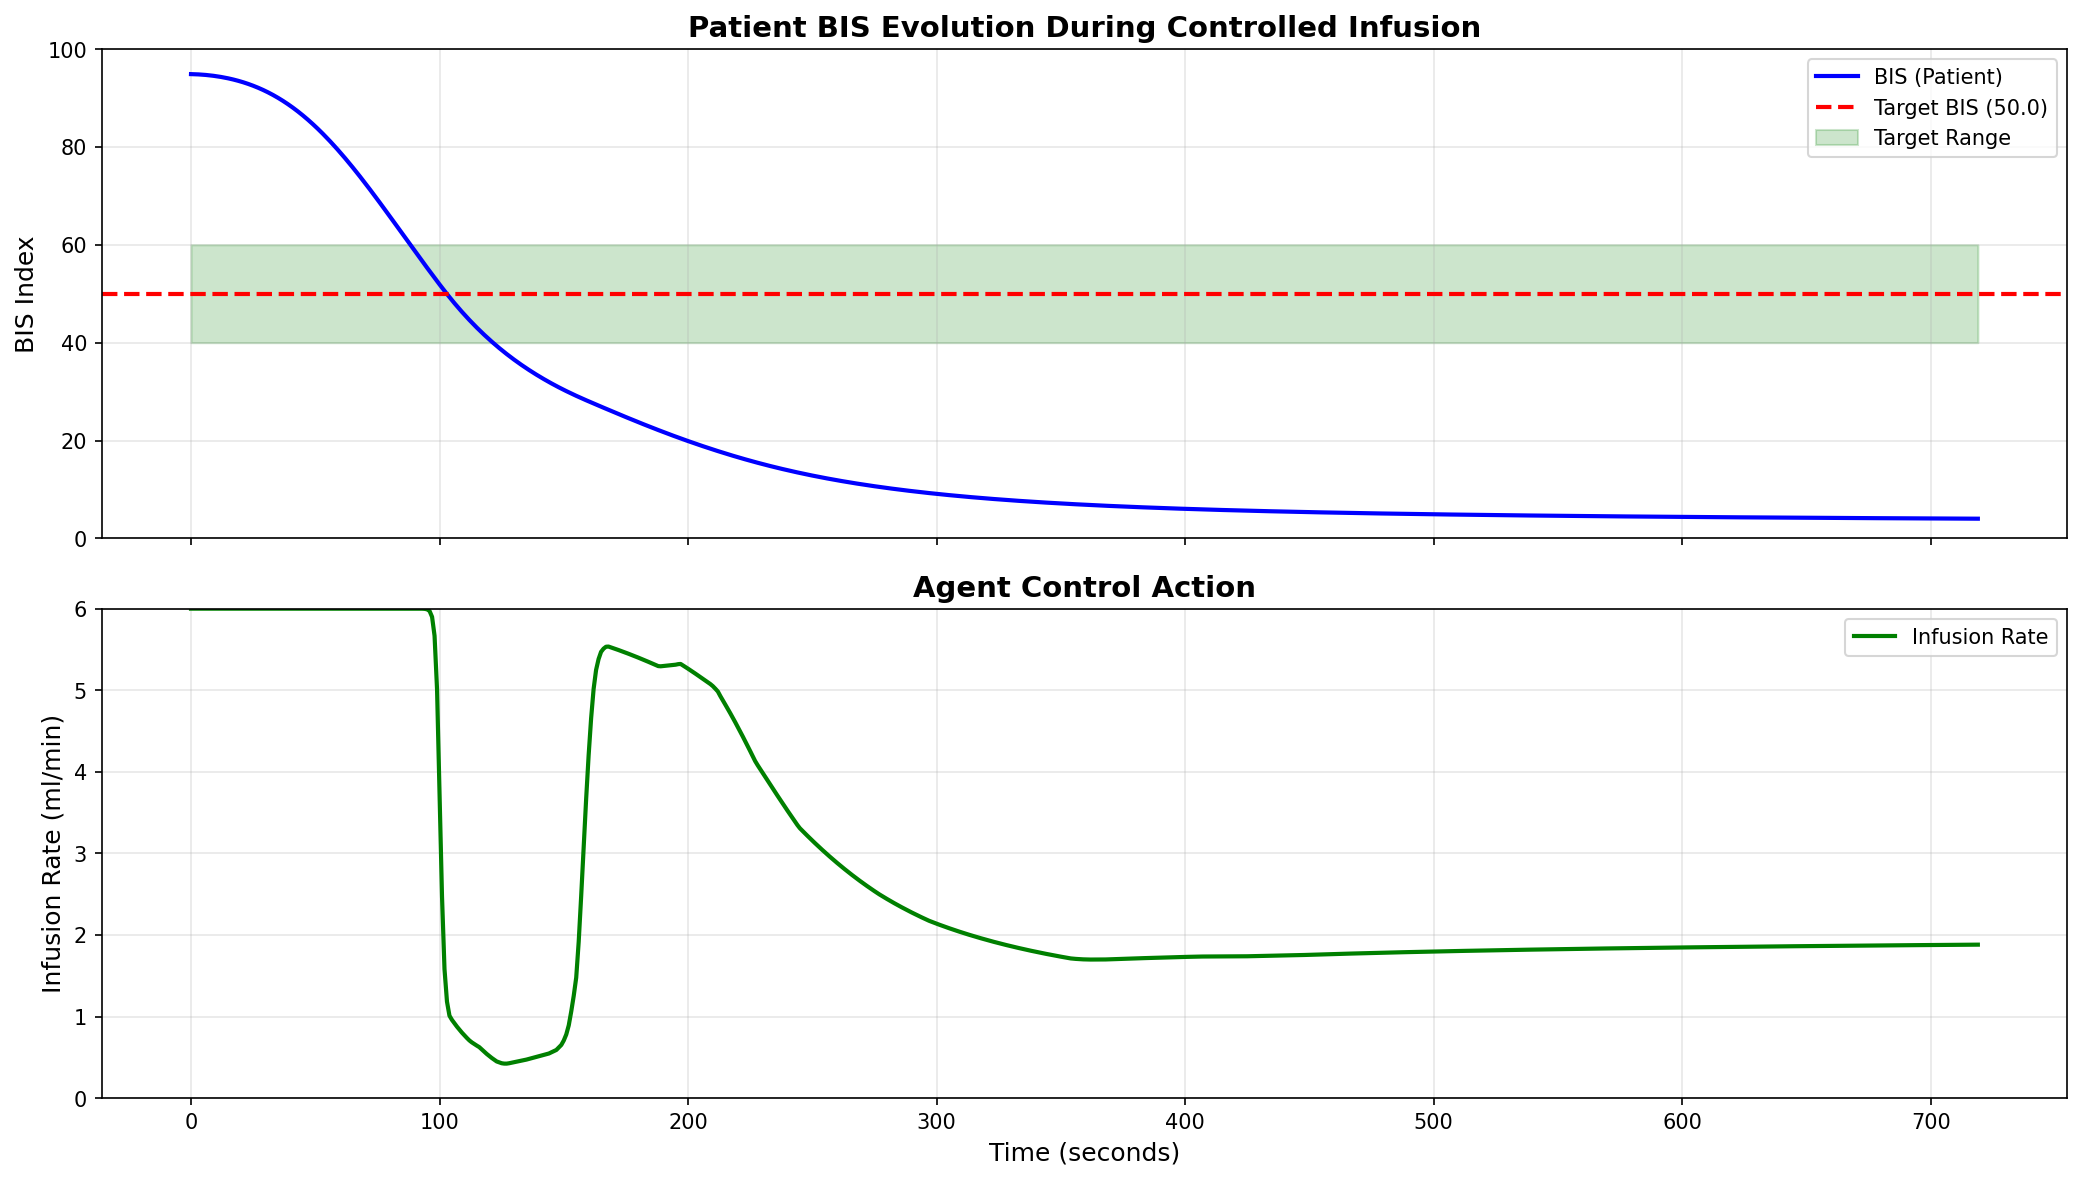
\includegraphics[width=0.85\textwidth]{images/bis_trajectory.png}
    \caption{Trajectoire BIS d'un patient exemple pendant la simulation}
    \label{fig:bis_traj}
\end{figure}

\clearpage

\subsection{Programmation Dynamique --- Itération de Politique}

L'Itération de Politique combine l'évaluation de politique avec l'amélioration itérative de politique. L'algorithme alterne entre le calcul des valeurs état-action via les transitions SARS' et l'extraction de la politique gloutonne.

\begin{figure}[htbp]
    \centering
    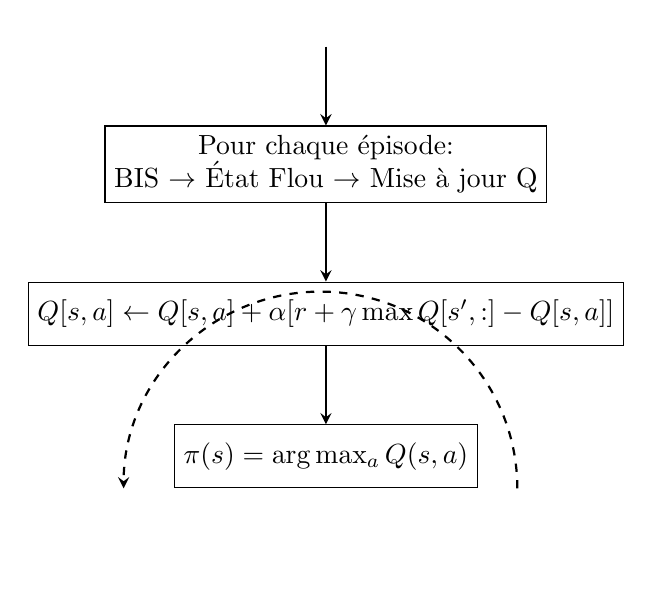
\begin{tikzpicture}[
        node distance=1cm,
        box/.style={rectangle, draw, minimum width=3cm, minimum height=0.8cm, align=center},
        arrow/.style={->, thick},
        >=stealth
    ]
    
    \node (start) {};
    \node (loop) [box, below=of start] {Pour chaque épisode:\\BIS $\rightarrow$ État Flou $\rightarrow$ Mise à jour Q};
    \node (update) [box, below=of loop] {$Q[s,a] \leftarrow Q[s,a] + \alpha[r + \gamma \max Q[s',:] - Q[s,a]]$};
    \node (extract) [box, below=of update] {$\pi(s) = \arg\max_a Q(s,a)$};
    \node (end) [below=of extract] {};
    
    \draw[arrow] (start) -- (loop);
    \draw[arrow] (loop) -- (update);
    \draw[arrow] (update) -- (extract);
    \draw[->, thick, dashed] ($(extract.south east) + (0.5,0)$) arc[start angle=0, end angle=180, radius=2.5cm];
    
    \end{tikzpicture}
    \caption{Boucle d'entraînement de l'Itération de Politique}
    \label{fig:policy_iter}
\end{figure}

\textbf{Hyperparamètres:} $\text{ÉPISODES} = 10{,}000$, $\text{PAS} = 120$, $\alpha = 0.2$, $\gamma = 0.69$, $\epsilon = 0.1$

\textbf{Statut d'entraînement:} Nécessite un entraînement supplémentaire. Le wobble élevé (21.71\%) indique une instabilité de contrôle.

\begin{figure}[htbp]
    \centering
    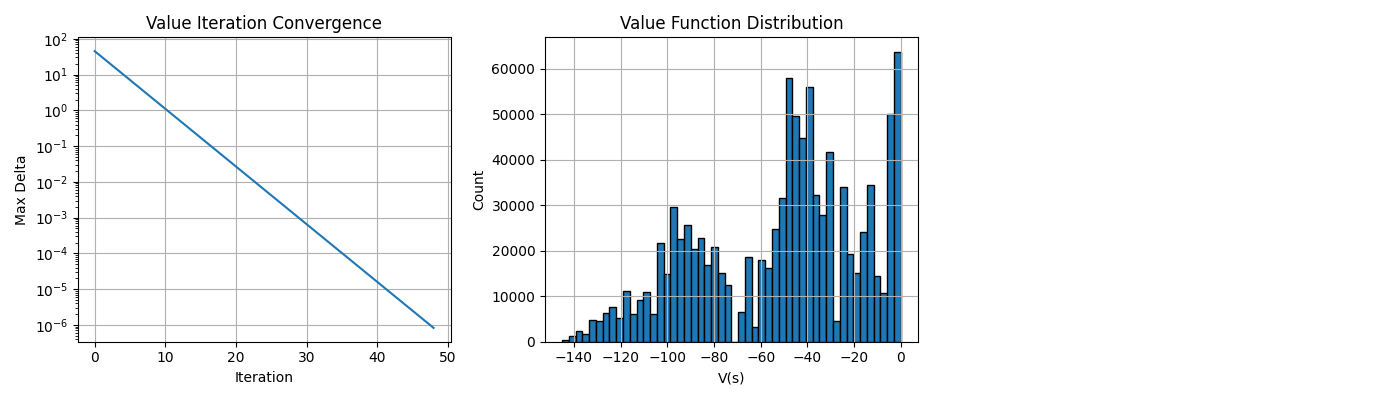
\includegraphics[width=0.85\textwidth]{images/dp_training_plots.png}
    \caption{Progrès de l'entraînement DP-Politique}
    \label{fig:dp_training}
\end{figure}

\begin{figure}[htbp]
    \centering
    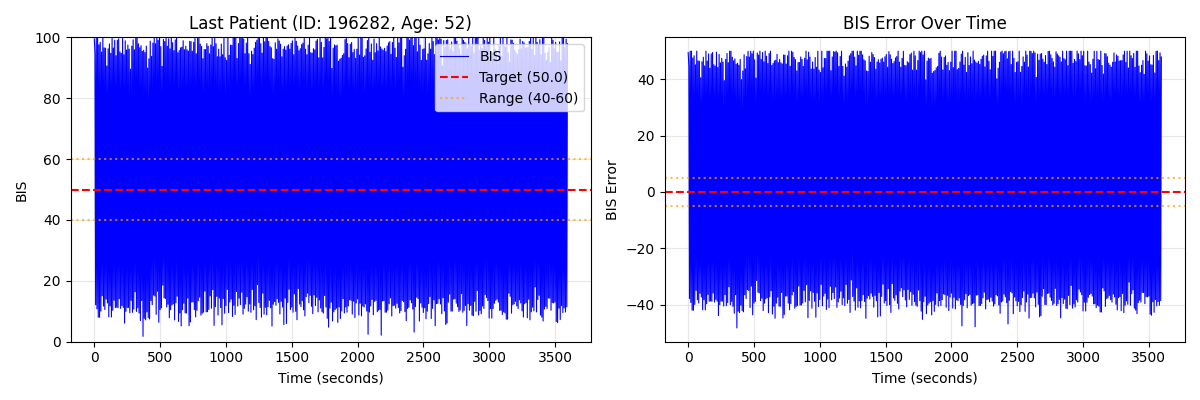
\includegraphics[width=0.85\textwidth]{images/dp_last_episode_plot.png}
    \caption{Comportement du dernier épisode d'entraînement}
    \label{fig:dp_episode}
\end{figure}

\begin{figure}[htbp]
    \centering
    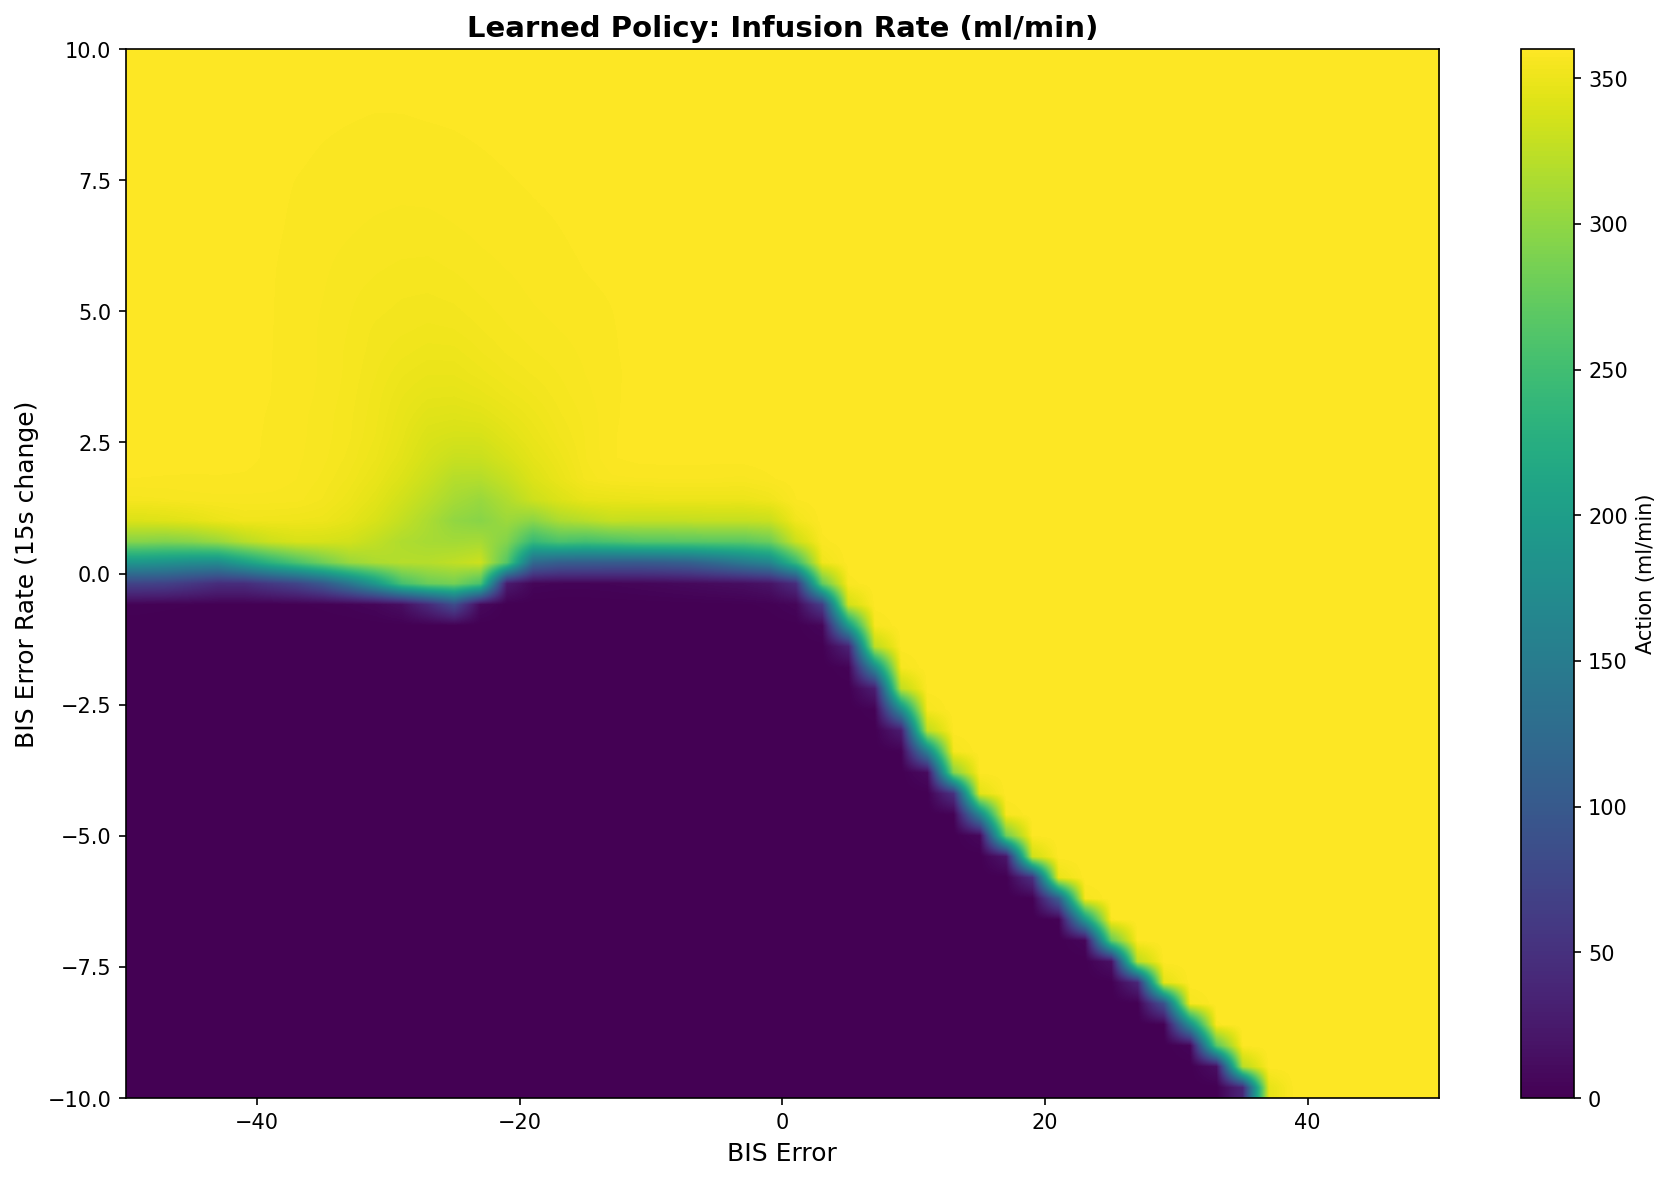
\includegraphics[width=0.85\textwidth]{images/policy_heatmap.png}
    \caption{Carte thermique de la politique apprise}
    \label{fig:policy_heatmap}
\end{figure}

\clearpage

\subsection{Programmation Dynamique --- Itération de Valeur}

L'Itération de Valeur calcule directement les valeurs optimales via l'équation d'optimalité de Bellman sur une matrice de transition précalculée. Cette approche suppose la connaissance de la dynamique de l'environnement.

\begin{figure}[htbp]
    \centering
    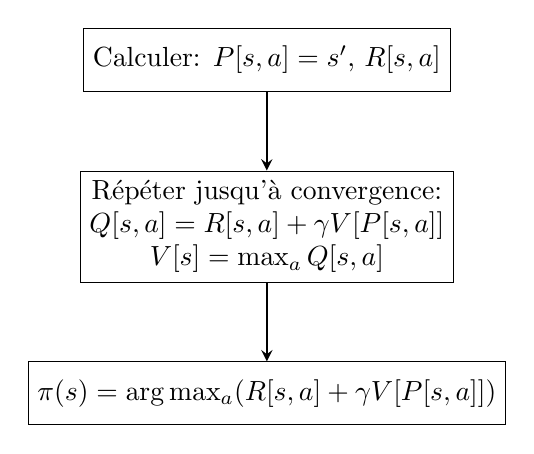
\begin{tikzpicture}[
        node distance=1cm,
        box/.style={rectangle, draw, minimum width=3.5cm, minimum height=0.8cm, align=center},
        arrow/.style={->, thick},
        >=stealth
    ]
    
    \node (transition) [box] {Calculer: $P[s,a] = s'$, $R[s,a]$};
    \node (iteration) [box, below=of transition] {Répéter jusqu'à convergence:\\$Q[s,a] = R[s,a] + \gamma V[P[s,a]]$\\$V[s] = \max_a Q[s,a]$};
    \node (policy) [box, below=of iteration] {$\pi(s) = \arg\max_a (R[s,a] + \gamma V[P[s,a]])$};
    
    \draw[arrow] (transition) -- (iteration);
    \draw[arrow] (iteration) -- (policy);
    
    \end{tikzpicture}
    \caption{Structure de l'algorithme d'Itération de Valeur}
    \label{fig:value_iter}
\end{figure}

\textbf{Hyperparamètres:} $\text{ITÉRATIONS} = 1{,}000{,}000$, $\gamma = 0.69$, $\epsilon = 0.1$

\textbf{Statut d'entraînement:} Partage la politique avec DP-Politique. Nécessite un entraînement supplémentaire.

\begin{figure}[htbp]
    \centering
    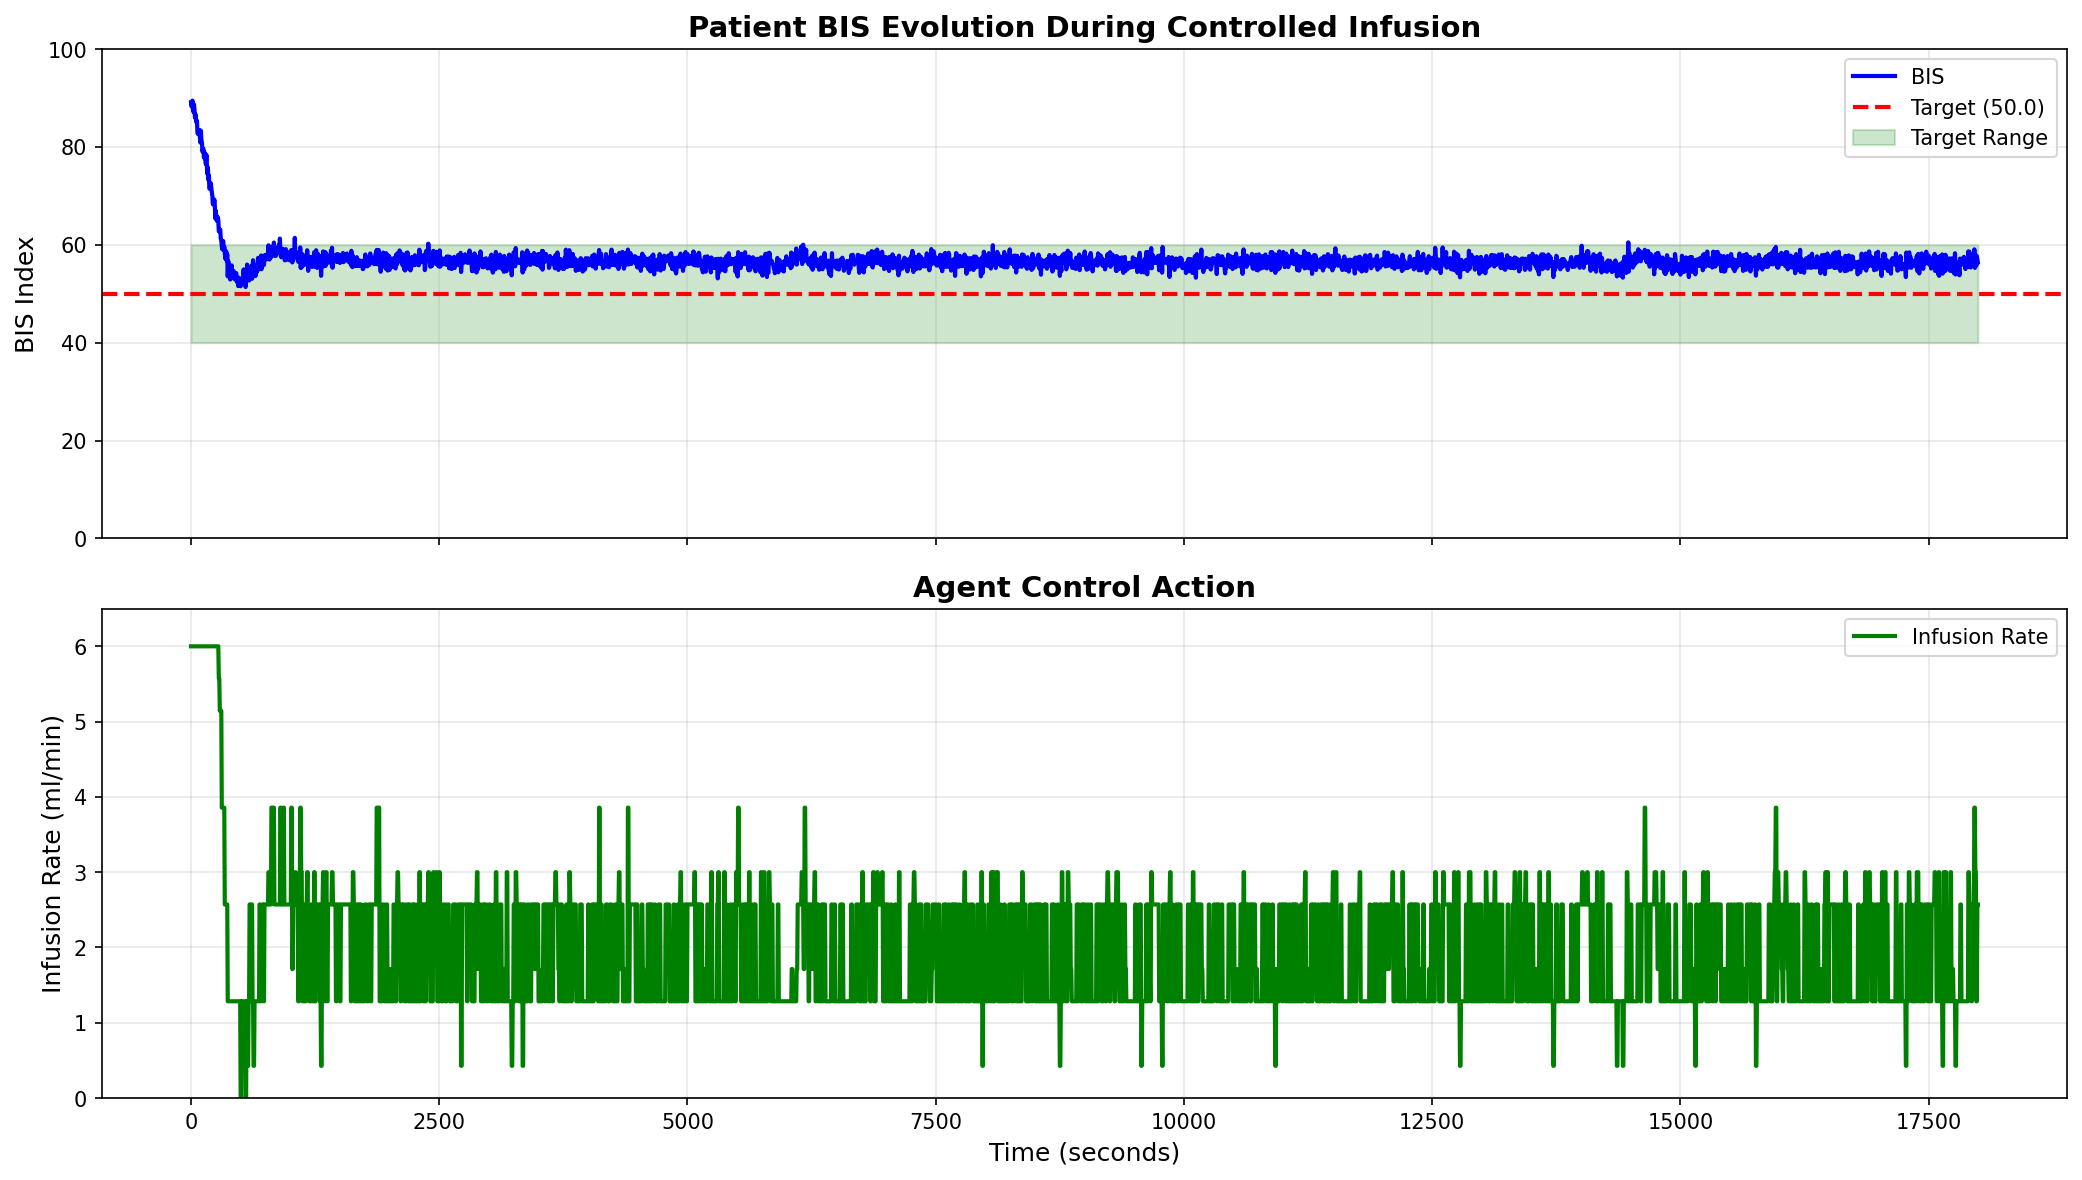
\includegraphics[width=0.85\textwidth]{images/dp_bis_trajectory.png}
    \caption{Trajectoire BIS sous la politique DP-Valeur}
    \label{fig:dpvalue_traj}
\end{figure}

\clearpage

\subsection{Deep Q-Network (DQN)}

DQN utilise un réseau de neurones pour approximer les valeurs Q, stabilisé par replay d'expérience et un réseau cible séparé.

\begin{figure}[htbp]
    \centering
    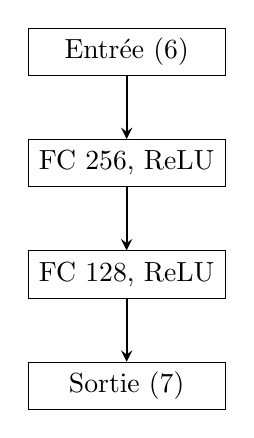
\begin{tikzpicture}[
        node distance=0.8cm,
        box/.style={rectangle, draw, minimum width=2.5cm, minimum height=0.6cm, align=center},
        arrow/.style={->, thick},
        >=stealth
    ]
    
    \node (input) [box] {Entrée (6)};
    \node (fc1) [box, below=of input] {FC 256, ReLU};
    \node (fc2) [box, below=of fc1] {FC 128, ReLU};
    \node (output) [box, below=of fc2] {Sortie (7)};
    
    \draw[arrow] (input) -- (fc1);
    \draw[arrow] (fc1) -- (fc2);
    \draw[arrow] (fc2) -- (output);
    
    \end{tikzpicture}
    \caption{Architecture du réseau neuronal DQN}
    \label{fig:dqn_net}
\end{figure}

\textbf{Architecture du réseau:} Entrée(6) $\rightarrow$ FC(256, ReLU) $\rightarrow$ FC(128, ReLU) $\rightarrow$ Sortie(7)

\textbf{Hyperparamètres:} $\text{ÉPISODES} = 10{,}000$, $\text{PAS} = 120$, $\text{LR} = 10^{-3}$, $\gamma = 0.69$, $\epsilon = 0.3 \rightarrow 0.01$, $\text{BUFFER} = 10{,}000$, $\text{BATCH} = 32$

\textbf{Statut d'entraînement:} Nécessite un entraînement supplémentaire. Performance similaire aux modèles DP.

\begin{figure}[htbp]
    \centering
    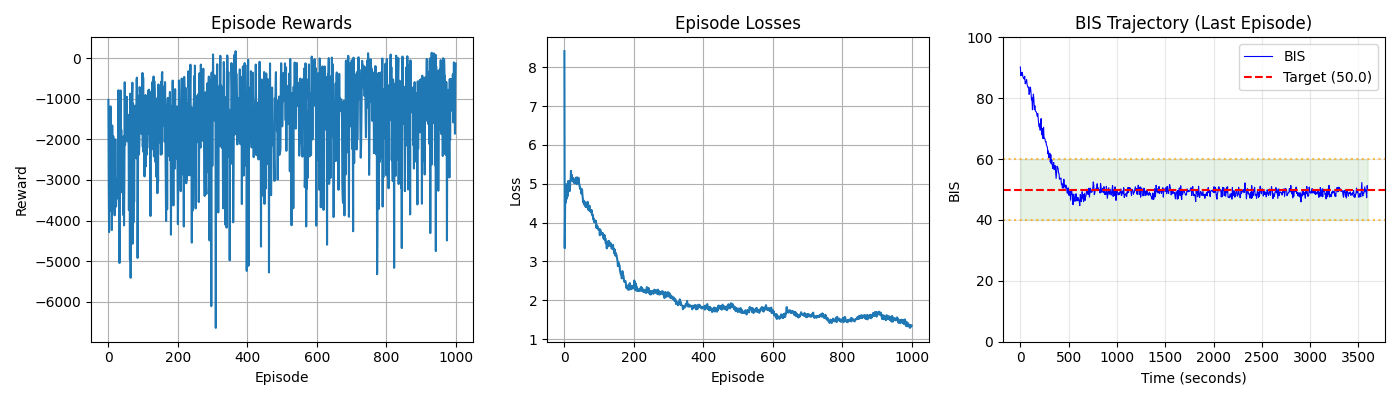
\includegraphics[width=0.85\textwidth]{images/dqn_training_plots.png}
    \caption{Courbes d'entraînement DQN: perte et décroissance d'epsilon}
    \label{fig:dqn_training}
\end{figure}

\begin{figure}[htbp]
    \centering
    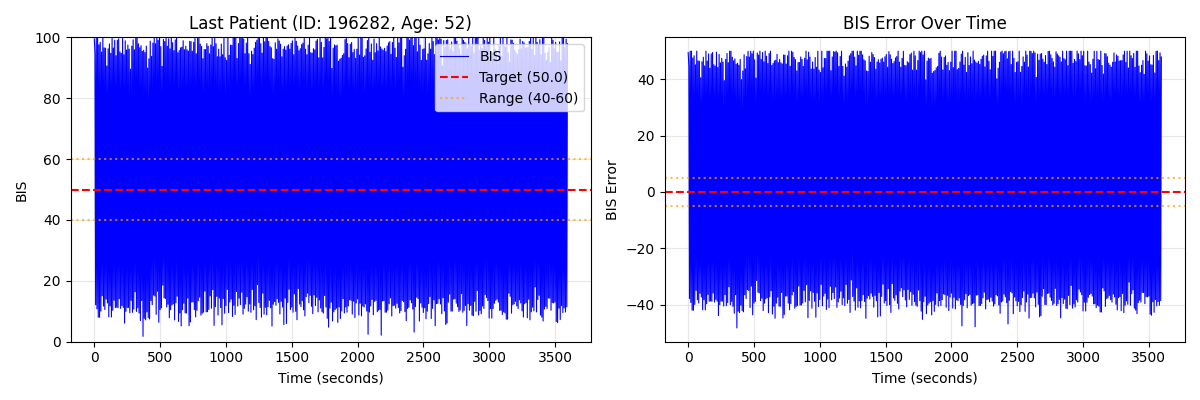
\includegraphics[width=0.85\textwidth]{images/dqn_last_episode_plot.png}
    \caption{Comportement du dernier épisode DQN}
    \label{fig:dqn_episode}
\end{figure}

\clearpage

\section{Modèle PK/PD: Schnider}

Le modèle de Schnider décrit la pharmacocinétique du propofol en utilisant un modèle mammifère à trois compartiments avec des paramètres estimés à partir de la démographie des patients.

\subsection{Paramètres des Compartiments}

\begin{table}[htbp]
    \centering
    \caption{Paramètres du modèle à compartiments}
    \begin{tabular}{lcl}
        \toprule
        \textbf{Paramètre} & \textbf{Valeur} & \textbf{Description} \\
        \midrule
        $V_1$ & \SI{4.27}{L} & Volume du compartiment central \\
        $V_2$ & \SI{18.9}{L} & Compartiment périphérique superficiel \\
        $V_3$ & \SI{238.0}{L} & Compartiment périphérique profond \\
        $k_{10}$ & 0.38 & Constante de vitesse d'élimination \\
        $k_{12}$ & 0.30 & Central $\rightarrow$ Superficiel \\
        $k_{21}$ & 0.20 & Superficiel $\rightarrow$ Central \\
        $k_{13}$ & 0.19 & Central $\rightarrow$ Profond \\
        $k_{31}$ & 0.0035 & Profond $\rightarrow$ Central \\
        $k_{e0}$ & 0.17 & Équilibration du site d'effet \\
        \bottomrule
    \end{tabular}
\end{table}

\subsection{Paramètres du Modèle BIS}

\begin{table}[htbp]
    \centering
    \caption{Paramètres du modèle d'effet BIS}
    \begin{tabular}{lcl}
        \toprule
        \textbf{Paramètre} & \textbf{Valeur} & \textbf{Description} \\
        \midrule
        $\text{BIS}_0$ & 95.0 & BIS de référence \\
        $\text{BIS}_{\max}$ & 75.0 & Effet BIS maximal \\
        $\text{EC}_{50}$ & \SI{3.5}{\micro\gram\per\mL} & EC50 à l'état stationnaire \\
        $\gamma$ (Hill) & 2.5 & Coefficient de Hill \\
        $\text{BIS}_{\text{target}}$ & 50.0 & BIS cible \\
        \bottomrule
    \end{tabular}
\end{table}

\clearpage

\section{Métriques d'Évaluation}

\begin{table}[htbp]
    \centering
    \caption{Définitions des métriques d'évaluation}
    \begin{tabular}{lp{10cm}}
        \toprule
        \textbf{Métrique} & \textbf{Description} \\
        \midrule
        MDPE & Erreur de Prédiction Médiane (\%); mesure le biais systématique \\
        MDAPE & Erreur de Prédiction Absolue Médiane (\%); mesure la précision \\
        Wobble & Déviation médiane par rapport à PE médian (\%); mesure la stabilité \\
        TimeInTarget & Pourcentage du temps dans $\pm5$ du BIS cible \\
        \bottomrule
    \end{tabular}
\end{table}

\section{Résultats}

\subsection{Performance Globale}

\begin{table}[htbp]
    \centering
    \caption{Comparaison de performance entre les algorithmes (durée 3600s)}
    \begin{tabular}{lcccc}
        \toprule
        \textbf{Modèle} & \textbf{MDPE (\%)} & \textbf{MDAPE (\%)} & \textbf{Wobble (\%)} & \textbf{TimeInTarget (\%)} \\
        \midrule
        Q-Learning & 94.79 & 94.79 & 4.05 & 0.0 \\
        DP-Politique & 78.35 & 86.25 & 21.71 & 0.0 \\
        DP-Valeur & 78.35 & 86.25 & 21.71 & 0.0 \\
        DQN & 78.35 & 86.25 & 21.71 & 0.0 \\
        \bottomrule
    \end{tabular}
\end{table}

\subsection{Performance par Groupe d'Âge}

\begin{table}[htbp]
    \centering
    \caption{Métriques de performance par groupe d'âge (durée 3600s)}
    \begin{tabular}{lcccc}
        \toprule
        \textbf{Groupe d'Âge} & \textbf{N} & \textbf{MDPE (\%)} & \textbf{MDAPE (\%)} & \textbf{Wobble (\%)} \\
        \midrule
        25--29 & 19 & 78.49 & 86.19 & 21.51 \\
        30--45 & 96 & 78.05 & 86.27 & 21.95 \\
        46--60 & 139 & 78.18 & 86.19 & 21.82 \\
        60--80 & 175 & 78.19 & 86.21 & 21.81 \\
        80+ & 38 & 78.56 & 86.30 & 21.44 \\
        \bottomrule
    \end{tabular}
\end{table}

\section{Conclusions}

Tous les modèles évalués nécessitent un entraînement supplémentaire pour atteindre un contrôle d'anesthésie cliniquement acceptable:

\begin{itemize}
    \item \textbf{Q-Learning:} Sévèrement sous-entraîné. Le MDPE élevé de 94.79\% indique que les valeurs BIS restent proches de la référence (95), suggérant une administration de propofol insuffisante. L'équilibre exploration-exploitation peut nécessiter un ajustement.
    
    \item \textbf{DP-Politique/Valeur:} Entraînement modéré atteint. Le wobble élevé (21.71\%) démontre une instabilité de contrôle avec des valeurs BIS oscillantes. La politique semble avoir du mal à maintenir un contrôle en régime permanent.
    
    \item \textbf{DQN:} Entraînement modéré atteint. La performance reflète les méthodes basées sur DP, suggérant que le réseau de neurones n'a pas encore appris de politiques de contrôle robustes.
\end{itemize}

\subsection{Prochaines Étapes Recommandées}

\begin{enumerate}
    \item Augmenter considérablement les épisodes d'entraînement pour tous les algorithmes
    \item Ajuster la fonction de récompense pour encourager une réduction plus rapide du BIS
    \item Optimiser les hyperparamètres (taux d'apprentissage, facteur d'actualisation, taux d'exploration)
    \item Envisager le reward shaping pour accélérer l'apprentissage initial
    \item Implémenter des stratégies d'apprentissage par curriculum
\end{enumerate}

\vfill

\section*{Remerciements}

Ce travail a été réalisé dans le cadre de la recherche sur les systèmes de contrôle automatisé de l'anesthésie.

\end{document}
